% ------------------------------------------------------------------------------
% TYPO3 CMS 7.3 - What's New (English Version)
%
% @author	Michael Schams <schams.net>
% @license	Creative Commons BY-NC-SA 3.0
% @link		http://typo3.org/download/release-notes/whats-new/
% @language	English
% ------------------------------------------------------------------------------
% LTXE-CHAPTER-UID:		cc6b358d-f0ed36d3-f7a72fa2-af63ccfc
% LTXE-CHAPTER-NAME:	Backend User Interface
% ------------------------------------------------------------------------------

\section{Administratorski interfejs}
\begin{frame}[fragile]
	\frametitle{Administratorski interfejs}

	\begin{center}\huge{Poglavlje 1:}\end{center}
	\begin{center}\huge{\color{typo3darkgrey}\textbf{Administratorski interfejs}}\end{center}

\end{frame}

% ------------------------------------------------------------------------------
% LTXE-SLIDE-START
% LTXE-SLIDE-UID:		51538163-e489db88-bc155df2-11f8948a
% LTXE-SLIDE-ORIGIN:	111332b8-ac46a07a-319ed582-f873bc02 English
% LTXE-SLIDE-ORIGIN:	b4dc1576-57b4854f-26a32d85-11f7c52b German
% LTXE-SLIDE-TITLE:		Feature #66173: Allow page title edit by doubleclick
% LTXE-SLIDE-REFERENCE:	Feature-66173-AllowPageTitleEditByDoubleclick.rst
% ------------------------------------------------------------------------------
\begin{frame}[fragile]
	\frametitle{Administratorski interfejs}
	\framesubtitle{Naslov strane u Page i List modulu}

	Korisnici mogu da menjaju naslove strana u "Page" i "List" modulu duplim klikom na zaglavlje strane ili ikonicu za izmenu.

	\begin{figure}
		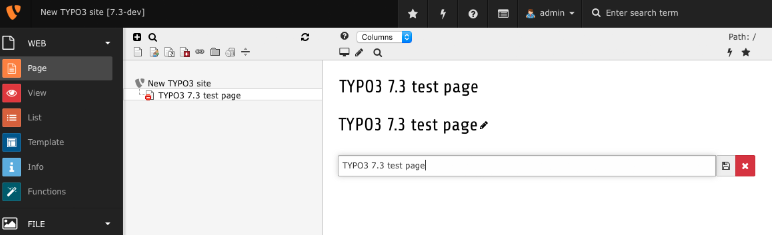
\includegraphics[width=0.9\linewidth]{BackendUserInterface/66173.png}
	\end{figure}

\end{frame}

% ------------------------------------------------------------------------------
% LTXE-SLIDE-START
% LTXE-SLIDE-UID:		96e7bc58-f2fb5838-5c9cb548-adbc0ac7
% LTXE-SLIDE-ORIGIN:	c17b263e-12512d4b-13d5389f-df1ec14e English
% LTXE-SLIDE-ORIGIN:	168b1424-1ebb2552-ed5bac3e-8a9ac737 German
% LTXE-SLIDE-TITLE:		Feature #67071: Processed files cleanup tool added in Install Tool
% LTXE-SLIDE-REFERENCE:	Feature-67071-ProcessedFilesCleanupToolAddedInInstallTool.rst
% ------------------------------------------------------------------------------
\begin{frame}[fragile]
	\frametitle{Administratorski interfejs}
	\framesubtitle{Install Tool: Brisanje obradjenih fajlova}

	U svojoj "Clean up" sekciji, Install Tool sada obezbedjuje novu funkciju za uklanjanje obradjenih fajlova (npr. thumbnails) iz FAL-a.\newline
	Ovo je korisno ukoliko su podesavanja vezana za slike promenjena ili, na primer, nakon azuriranja GraphicsMagick/ImageMagick-a kako bi se isforsiralo da sve slike budu ponovo generisane.

	\begin{figure}
		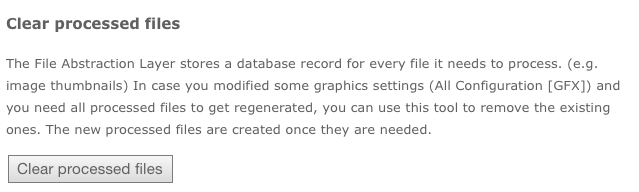
\includegraphics[width=0.6\linewidth]{BackendUserInterface/67071.png}
	\end{figure}

\end{frame}

% ------------------------------------------------------------------------------
% LTXE-SLIDE-START
% LTXE-SLIDE-UID:		54d0d5fb-83798bed-760aa086-20c75556
% LTXE-SLIDE-ORIGIN:	4662a0fc-e8a91f22-2f75e0bc-800e9b63 English
% LTXE-SLIDE-ORIGIN:	daa83c1e-08d2716b-de74cbda-42361551 German
% LTXE-SLIDE-TITLE:		Feature #67319: Add field "copyright" to EXT:filemetadata
% LTXE-SLIDE-REFERENCE:	Feature-67319-AddFieldCopyrightToEXTfilemetadata.rst
% ------------------------------------------------------------------------------
\begin{frame}[fragile]
	\frametitle{Administratorski interfejs}
	\framesubtitle{Novo polje u FAL Meta podacima}

	Polje "\textbf{Copyright}" dodato je u meta podatke FAL rekorda 
	(sistemsko prosirenje: \texttt{filemetadata}).

	\begin{figure}
		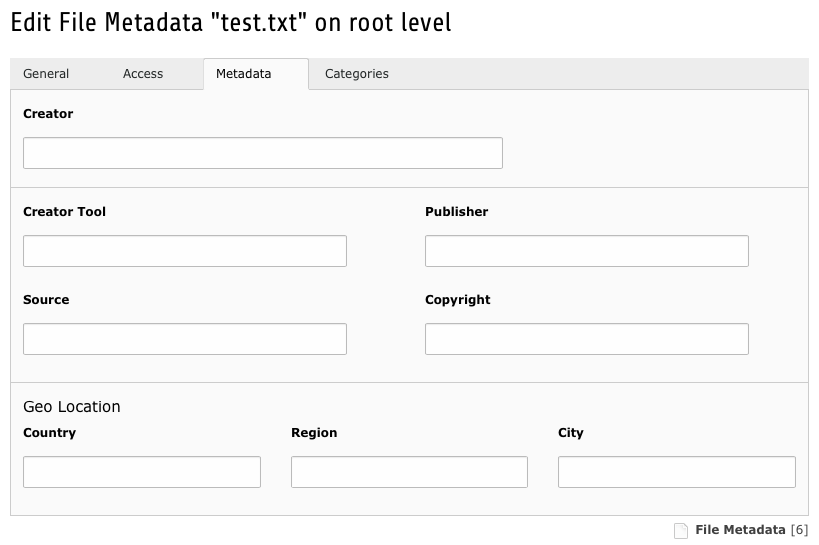
\includegraphics[width=0.6\linewidth]{BackendUserInterface/67319.png}
	\end{figure}

\end{frame}

% ------------------------------------------------------------------------------
